\documentclass[]{article}
\usepackage{geometry}   % my added package "geometry"
\geometry{letterpaper,tmargin=1in,bmargin=1in,lmargin=2.2cm,rmargin=2.2cm}
\usepackage[colorlinks,bookmarksopen,bookmarksnumbered,
citecolor=green,urlcolor=red]{hyperref}
\hypersetup{pdfauthor={Name}}
%%%%%%%%%%%%%%%%%%%%%%%%%%%%%%%%%%%%%%%%%%%%%%%%%%%%%%%%%%%%%%%%%%%%%%%%%
%\usepackage{graphicx}
\usepackage{graphics}
\usepackage{epsfig}
\usepackage{epstopdf}
\usepackage{amsfonts}
\usepackage{amssymb}
\usepackage{booktabs}
\usepackage{color,soul}
%%%%%%%%%%%%%%%%%%%%%%%%%%%%%%%%%%%%%%%%%%%%%%%%%%%%%%%%%%%%%%%%%
\usepackage{amsmath}
\usepackage{cleveref}
%\usepackage[fleqn]{amsmath}
\usepackage{lineno}
\usepackage{tikz}
\usepackage{standalone}
\usetikzlibrary{calc,patterns,arrows.meta,shapes.arrows,intersections,positioning}
\usetikzlibrary{decorations.pathmorphing,backgrounds,fit,petri}
\usepackage[percent]{overpic}
%%%%%%%%%%%%%%%%%%%%%%%%%%%%%%%%%%%%%%%%%%%%%%%%%%%%%%%%%%%%%%%%%
\usepackage{xcolor}
\usepackage{listings}
\lstset { %
	language=C++,
	backgroundcolor=\color{blue!5}, % set backgroundcolor
	basicstyle=\footnotesize\color{black},% basic font settingbasicstyle=\ttfamily\color{black}
	keywordstyle=\color{red},
	commentstyle=\color{violet},
	stringstyle=\color{blue},
	xleftmargin=2em,
	frame=single,
	framexleftmargin=2em,
	numbers=left,
	numberstyle=\tiny,
	numbersep=8pt,
}
%%%%%%%%%%%%%%%%%%%%%%%%%%%%%%%%%%%%%%%%%%%%%%%%%%%%%%%%%%%%%%%%%
\renewcommand\thesubsection{\thesection\Alph{subsection}}
%%%%%%%%%%%%%%%%%%%%%%%%%%%%%%%%%%%%%%%%%%%%%%%%%%%%%%%%%%%%%%%%%
\renewcommand\lstlistingname{Header}
\renewcommand\lstlistlistingname{Header}
%%%%%%%%%%%%%%%%%%%%%%%%%%%%%%%%%%%%%%%%%%%%%%%%%%%%%%%%%%%%%%%%%%%%
%opening
\begin{document}
\title{HiperLife Tutorial: NonLinear Poisson}
\author{LaCàN}
\maketitle

\linenumbers

\section{Problem Definition} \label{sec: pd} 
Now we address how to solve nonlinear PDEs. Our sample PDE for implementation is taken as a nonlinear Poisson equation:\cite{BarattaEtal2023}
\begin{equation}\label{eq1}
	\begin{aligned}
		 - \nabla \cdot [(1+u)\nabla u] = f \quad \text{in} \ \Omega
	\end{aligned}
\end{equation}
As it is demonstrated in Figure \ref{fig_SB}, The domain $\Omega$ is a rectangle of dimensions $[0,1] \times [0,1]$ along the $x$ and $y$ coordinates, where $f = 0$ and the boundary conditions to be
\begin{equation}\label{eq2}
	\begin{aligned}
		u(0,y) &= 0, \ u(1,y) = 1\quad \text{on} \ \Gamma_D \\
		u_y(x,0) &=u_y(x,1) =0 \quad \text{on} \ \Gamma_N \\
	\end{aligned}
\end{equation}
\begin{figure}[htbp]
	\centering
	
\documentclass[preprint,12pt,a4]{standalone}
\usepackage{geometry}   % my added package "geometry"
\geometry{letterpaper,tmargin=1in,bmargin=1in,lmargin=2.5cm,rmargin=2.5cm}
\usepackage{tikz}
\usetikzlibrary{calc,patterns,arrows.meta,shapes.arrows,intersections,positioning}
\usetikzlibrary{decorations.pathmorphing,backgrounds,fit,petri}
\usepackage{standalone}
\begin{document}
	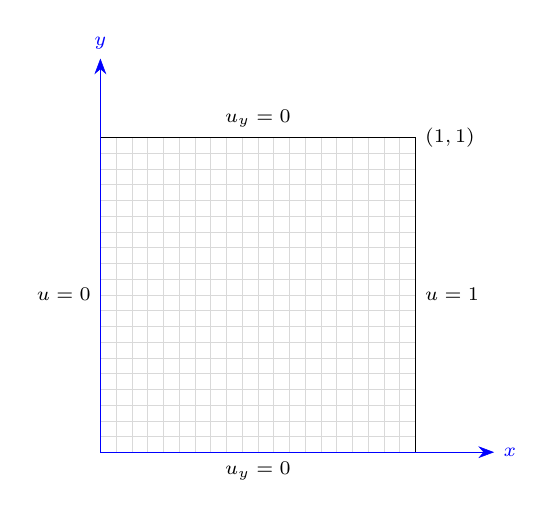
\begin{tikzpicture} [{place/.style={rectangle,draw=blue!50,fill=blue!20,ultra thin,inner sep=0.8mm}},{place2/.style={circle,draw=black!50,ultra thin,inner sep=0.8mm}},{linest/.style={color=gray,ultra thin}}]
	%%coordinates of corners of Beam
	\coordinate (A) at (0,0);
	\coordinate (B) at (2,0);
	\coordinate (C) at (4,0);
	\coordinate (D) at (4,2);
	\coordinate (E) at (4,4);
	\coordinate (F) at (2.0,4);
	\coordinate (G) at (0.0,4);
	\coordinate (H) at (0.0,2);
	%%mesh
	\draw [line width=0.1pt,gray!30,step=2mm](A) grid (E);
	%%Beam	
	\draw [color=black](A)-- (B)node [below,color = black,font=\scriptsize] {$u_y=0$}--(C)--(D)node [right,color = black,font=\scriptsize] {$u=1$}--(E)node [right,color = black,font=\scriptsize] {$(1,1)$}--(F)node [above,color = black,font=\scriptsize] {$u_y=0$}--(G)--(H)node [left,color = black,font=\scriptsize] {$u=0$}--(A);
	
	%%axes
	\draw [-{Stealth[length=2mm]},help lines,blue] (A) -> (5,0) node [right,color = blue,font=\scriptsize] {$x$};
		\draw [-{Stealth[length=2mm]}, help lines,blue] (A) -- (0,5) node [above,color = blue,font=\scriptsize] {$y$};

	\end{tikzpicture}
\end{document}
	\caption{Illustration of the domain of Poisson problem.}
	\label{fig_SB}
\end{figure}

The exact solution is then
\begin{equation}\label{eq3}
	\begin{aligned}
		u(x,y) = (3x +1)^{1/2}-1\thinspace .
	\end{aligned}
\end{equation}
We choose a uniform mesh of size $10 \times 10$ and quadrilateral Elements consist of four nodes to model the domain.
\section{Weak Form} \label{sec: WF}
The variational formulation of our model problem reads: Find $u \in V$ such that
\begin{equation}\label{eq4}
	\begin{aligned}
		\mathcal{F}(u;v) = 0 \quad \forall v \in \hat{V}
		\end{aligned}
\end{equation}
where
\begin{equation}\label{eq5}
	\begin{aligned}
		\mathcal{F}(u; v) =-\int_\Omega v \nabla \cdot[(1+u) \nabla u] - v f \mathrm{d}\Omega\thinspace .
		\end{aligned}
\end{equation}
and
\begin{equation}\label{eq6}
	\begin{aligned}
		\hat{V} &= \{v \in H^1(\Omega) : v = 0 \text{ on } x=0\mbox{ and }x=1\}, \\
		 V &= \{v \in H^1(\Omega) : v = 0 \text{ on } x=0\text{ and } v = 1\text{ on }x=1\}\thinspace.
		\end{aligned}
\end{equation}
The discrete problem arises as usual by restricting $V$ and $\hat{V}$ to a pair of discrete spaces. Since $\mathcal{F}$ is a nonlinear function of $u$, the variational statement gives rise to a system of nonlinear algebraic equations. using integrating by part this expression over $\Omega$, we have
\begin{equation}\label{eq8}
	\begin{aligned}
		\mathcal{F}(u; v) = -\int_{\Omega} \nabla \cdot [v (1+u) \nabla u] + \int_{\Omega}  (1+u)\nabla v\nabla u - \int_{\Omega} v f \mathrm{d}\Omega\thinspace .
	\end{aligned}
\end{equation}
Using Gauss’s theorem we get
\begin{equation}\label{eq9}
	\begin{aligned}
		\mathcal{F}(u; v) =  -\int_{\Gamma} [v (1+u^2) \nabla u] \cdot n \ \mathrm{d} \Gamma + \int_{\Omega} (1+u)\nabla u \nabla v \mathrm{d} \Omega - \int_{\Omega} v f \mathrm{d} \Omega\thinspace .
	\end{aligned}
\end{equation}
Applying boundary conditions ($\Gamma = \Gamma_N \cup \Gamma_D$):
\begin{equation}\label{eq10}
	\begin{aligned}
		v= 0 \quad &\text{ on } \Gamma_D\thinspace, \\
		\nabla u \cdot n = 0 \quad &\text{ on } \Gamma_N \thinspace.
	\end{aligned}
\end{equation}

and assuming $f=0$ we get the final form for $\mathcal{F}$
\begin{equation}\label{eq11}
	\begin{aligned}
		\mathcal{F}(u; v) = \int_\Omega (1+u)\nabla u\cdot \nabla v \, \mathrm{d}\Omega,
	\end{aligned}
\end{equation}
After having discretized our nonlinear PDE problem, we now need to linearize it, we may use Newton’s method to solve the system of nonlinear algebraic equations. Newton’s method for the system $\mathcal{F}_i(U_1,\ldots,U_j)=$ can be formulated by the first terms of a Taylor series approximation for the value of the variational as
\begin{equation}\label{eq12}
	\begin{aligned}
		\sum_{j=1}^N {\partial \over\partial U_j} \mathcal{F}_i(U_1^k,\ldots,U_N^k)\delta U_j &= -\mathcal{F}_i(U_1^k,\ldots,U_N^k),\quad i=1, \ldots ,N,\\ U_j^{k+1} &= U_j^k + \delta U_j,\quad j=1, \ldots ,N,
	\end{aligned}
\end{equation}
where $k$ is an iteration index. An initial guess $u^0$ must be provided to start the algorithm.
We need to compute the $\partial \mathcal{F}_i/\partial U_j$ and the right-hand side vector $-\mathcal{F}_i$. Our present problem has $\mathcal{F}_i$ given by above. Since $u = \sum_{j=1}^N U_j \phi_j$ the jacobian ($\mathcal{J}=\partial \mathcal{F}_i/\partial U_j$) can be introduced in this way
\begin{equation}\label{eq13}
	\begin{aligned}
		\mathcal{J}(u;\phi_j,\phi_i) = {\partial F_i\over\partial U_j} = \int_\Omega \left\lbrack \phi_j \nabla u^k \cdot \nabla \phi_i + (1+u^k) \nabla \phi_j \cdot \nabla \phi_i \right\rbrack \, \mathrm{d}\Omega\thinspace .
	\end{aligned}
\end{equation}
The elemental representation of the vector and matrix required for implementation in hiperlife would be like\footnote{Note that HiperLife by default applies the $-$ in $Bk(i)$ in Nonlinear problems, so it is not required to add it in your code!}
\begin{equation}\label{eq14}
	\begin{aligned}[b]
		Bk(i) &= -\mathcal{F}_i = \mathcolor{red}{-}jac \times[(1+u^k)\nabla u^k\cdot \nabla \phi_i], \\
		Ak(i,j) &=  \mathcal{J}_{ij} = jac \times [\phi_j \nabla u^k \cdot \nabla \phi_i + (1+u^k) \nabla \phi_j \cdot \nabla \phi_i]\thinspace .
	\end{aligned}
\end{equation}

\section{Implementation} \label{sec: imp}
In this section, we present the implementation of our solution in the Hiperlife. The program is divided into three separate files, main part which we create our problem by the Hiperlife headers, auxiliary header where we introduce parameters and declare defined functions, and at last auxiliary file, where we define some functions which provide required matrices like the Jacobian and the Hessian.
\subsubsection{PoissonNonL.cpp} \label{sec: m.cpp}
\nolinenumbers
\begin{lstlisting}
/*
* nonlinear Poisson equation (using nonlinear solver)
*/

// C++ headers
#include <iostream>
#include <fstream>
#include <time.h>

// hiperlife headers
#include "hl_Core.h"
#include "hl_Parser.h"
#include "hl_TypeDefs.h"  
#include "hl_DOFsHandler.h"
#include "hl_HiPerProblem.h"
#include "hl_SurfLagrParam.h"
#include "hl_FillStructure.h"
#include "hl_ParamStructure.h"
#include "hl_DistributedMesh.h" 
#include "hl_StructMeshGenerator.h" 
#include "hl_GlobalBasisFunctions.h"
#include "hl_NonlinearSolver_NewtonRaphson.h"
#include "hl_LinearSolver_Iterative_AztecOO.h"
#include <hl_ConsistencyCheck.h>


// problem header
#include "AuxPoissonNonL.h"

int main(int argc, char** argv)
{
	using namespace std;
	using namespace hiperlife;
	
	// **************************************************************//
	/// *****                 INITIALIZATION                    **** ///
	// **************************************************************//
	
	// Initialize the MPI execution environment
	hiperlife::Init(argc, argv);
	
	// Define parameters of the model
	SmartPtr<ParamStructure> paramStr = CreateParamStructure<PoissonParams>();
	double f  = paramStr->getRealParameter(PoissonParams::f);
	
	// **************************************************************//
	// *****                  MESH CREATION                     *****//
	// **************************************************************//
	
	// Create structured mesh
	SmartPtr<StructMeshGenerator> mesh = Create<StructMeshGenerator>();
	mesh->setNDim(3);
	mesh->setElemType(ElemType::Square);
	mesh->setBasisFuncType(BasisFuncType::Lagrangian);
	mesh->setBasisFuncOrder(1);
	mesh->genSquare(10,1.0);
	
	// Distributed mesh
	SmartPtr<DistributedMesh> disMesh = Create<DistributedMesh>();
	disMesh->setMesh(mesh);
	disMesh->setBalanceMesh(true);
	disMesh->setElementLocatorEngine(ElementLocatorEngine::BoundingVolumeHierarchy);
	disMesh->Update();
	
	// checking mesh
	disMesh->printFileLegacyVtk("mesh");
	
	// **************************************************************//
	// *****               DOFsHANDLER CREATION                 *****//
	// **************************************************************//
	
	// Create DOFsHandler
	SmartPtr<DOFsHandler> dofHand = Create<DOFsHandler>(disMesh);
	dofHand->setNameTag("dofHand");
	dofHand->setNumDOFs(1);
	dofHand->setDOFs({"u"});
	dofHand->Update();
	
	// -------------- initial condition first guess ----------------- //
	//----------------------------------------------------------------//
	for (int i = 0; i < disMesh->loc_nPts(); i++)
	{
		// Coordinate
		std::vector<double> x = disMesh->nodeCoords(i, IndexType::Local);
		// Initial condition
		dofHand->nodeDOFs->setValue("u", i, IndexType::Local, x[0]);
		// ---------------------- Boundary condition ---------------- //
		//------------------------------------------------------------//
		if (x[0] < 1e-5)
		{
			dofHand->nodeDOFs->setValue("u", i, IndexType::Local,0.0);
			dofHand->setConstraint("u",i, IndexType::Local,0.0);
		}
		if (x[0] > (1.-1e-5))
		{
			dofHand->nodeDOFs->setValue("u", i, IndexType::Local,1.0);
			dofHand->setConstraint("u",i, IndexType::Local,0.0);
		}
	}
	
	// Update 
	dofHand->UpdateGhosts();
	
	// checking initial and boundary condition
	dofHand->printFileLegacyVtk("PoissonNonL0");
	
	// *************************************************************  //
	/// *****               HIPERPROBLEM CREATION               **** ///
	// *************************************************************  //
	
	// Create hiperproblem
	SmartPtr<HiPerProblem> hiperProbl = Create<HiPerProblem>();
	
	// Set parameter structure and DOFsHandler
	hiperProbl->setParameterStructure(paramStr);
	hiperProbl->setDOFsHandlers({dofHand});
	
	// Set integration in the bulk
	hiperProbl->setIntegration("Integ", {"dofHand"});
	hiperProbl->setCubatureGauss("Integ",4);
	hiperProbl->setElementFillings("Integ", LS);
	
	// Consistency Check
	if (true)
	{
		hiperProbl->setConsistencyDOFs("dofHand", {"u"});
		hiperProbl->setElementFillings("Integ", ConsistencyCheck<LS>);
		hiperProbl->setConsistencyCheckType(ConsistencyCheckType::Hessian);
	}
	
	// Update
	hiperProbl->Update();
	
	
	// ************************************************************** //
	/// ****                SOLVE HIPERPROBLEM                  **** ///
	// ************************************************************** //
	
	// Create linear solver
	SmartPtr<AztecOOIterativeLinearSolver> linsolver = Create<AztecOOIterativeLinearSolver>();
	linsolver->setHiPerProblem(hiperProbl);
	linsolver->setTolerance(1.E-8);
	linsolver->setMaxNumIterations(500);
	linsolver->setSolver(AztecOOIterativeLinearSolver::Solver::Gmres);
	linsolver->setPreconditioner(AztecOOIterativeLinearSolver::Preconditioner::None);
	linsolver->setDefaultParameters();
	linsolver->setVerbosity(AztecOOIterativeLinearSolver::Verbosity::None);
	linsolver->Update();
	
	// Create nonlinear solver
	SmartPtr<NewtonRaphsonNonlinearSolver> nonLinSolver = Create<NewtonRaphsonNonlinearSolver>();
	nonLinSolver->setLinearSolver(linsolver);
	nonLinSolver->setConvRelTolerance(true);
	nonLinSolver->setMaxNumIterations(15);
	nonLinSolver->setResTolerance(1e-6);
	nonLinSolver->setSolTolerance(1e-6);
	nonLinSolver->setResMaximum(1e5);
	nonLinSolver->setSolMaximum(1e5);
	nonLinSolver->setExitRelMaximum(true);
	nonLinSolver->setLineSearch(false);
	nonLinSolver->setPrintSummary(false);
	nonLinSolver->setPrintIntermInfo(true);
	nonLinSolver->Update();
	
	// Solve
	bool converged = nonLinSolver->solve();
	
	// Check convergence
	if (converged)
	{
		// Save solution
		dofHand->nodeDOFs0->setValue(dofHand->nodeDOFs);
		dofHand->nodeDOFs0->UpdateGhosts();
		
		// Print solution
		dofHand->printFileLegacyVtk("PoissonNonL");
	}
	
	// ***************************************************************//
	/// ****                   FINALIZE                          ****///
	// ***************************************************************//
	hiperlife::Finalize();
	return 0;
}

\end{lstlisting}
\subsubsection{AuxPoissonNonL.h} \label{sec: a.h}
\begin{lstlisting}
#ifndef AUXPoisson_H
#define AUXPoisson_H

// C headers
#include <iostream>

// hiperlife headers
#include "hl_Core.h"
#include "hl_ParamStructure.h"
#include "hl_Parser.h"
#include "hl_TypeDefs.h"
#include "hl_MeshLoader.h"
#include "hl_StructMeshGenerator.h"
#include "hl_DistributedMesh.h"
#include "hl_FillStructure.h"
#include "hl_DOFsHandler.h"
#include "hl_HiPerProblem.h"
#include "hl_SurfLagrParam.h"
#include "hl_LinearSolver_Iterative_AztecOO.h"
#include "hl_GlobalBasisFunctions.h"
#include "hl_NonlinearSolver_NewtonRaphson.h"

struct PoissonParams
{
	enum RealParameters
	{
		f
	};
	enum StringParameters
	{
		filemesh
	};
	HL_PARAMETER_LIST DefaultValues
	{
		{"f", 0.0},
		{"filemesh", ""},
	};
};


void LS(hiperlife::FillStructure& fillStr);

#endif

\end{lstlisting}
\subsubsection{AuxPoissonNonL.cpp} \label{sec: a.cpp}
\begin{lstlisting}
// hiperlife headers
#include "hl_Core.h"
#include "hl_ParamStructure.h"
#include "hl_Parser.h"
#include "hl_TypeDefs.h"
#include "hl_MeshLoader.h"
#include "hl_StructMeshGenerator.h"
#include "hl_DistributedMesh.h"
#include "hl_FillStructure.h"
#include "hl_DOFsHandler.h"
#include "hl_HiPerProblem.h"
#include "hl_SurfLagrParam.h"
#include "hl_LinearSolver_Iterative_AztecOO.h"
#include "hl_GlobalBasisFunctions.h"
#include "hl_NonlinearSolver_NewtonRaphson.h"
// problem header
#include "AuxPoissonNonL.h"

void LS(hiperlife::FillStructure& fillStr)
{
	using namespace std;
	using namespace hiperlife;
	using hiperlife::Tensor::tensor;
	
	// Dimensions
	SubFillStructure& subFill = fillStr["dofHand"];
	int nDOFs = subFill.numDOFs;                                        
	int eNN   = subFill.eNN;                                           
	int nDim  = subFill.nDim;                                        
	int pDim  = subFill.pDim;
	
	// Nodal values at Gauss points
	vector<double>& nborCoords = subFill.nborCoords; // Vector of node coordinates
	ttl::wrapper<double,1> nborDOFs(subFill.nborDOFs.data(),eNN);
	
	// Shape functions and derivatives at Gauss points
	double jac; 
	ttl::wrapper<double,1>  bf(subFill.nborBFs(), eNN);
	tensor<double,2> Dbf(eNN,pDim); 
	GlobalBasisFunctions::gradients(Dbf, jac, subFill);
	
	// source
	double f = fillStr.getRealParameter(PoissonParams::f);
	
	//-----------------------------------------------------------------//
	//--------------------- OUTPUT DATA -------------------------------//
	//-----------------------------------------------------------------//
	ttl::wrapper<double,2> Ak(fillStr.Ak(0, 0).data(), eNN, eNN);
	ttl::wrapper<double,1> Bk(fillStr.Bk(0).data(),eNN);
	
	//=====================  previous step values =====================//
	// u
	double u = bf*nborDOFs;
	// grad u
	tensor<double,1> gradu(pDim);
	for (int i = 0; i < eNN; i++)
	{
		for (int d = 0; d < pDim; d++)
		gradu(d) += Dbf(i,d)*nborDOFs(i); 
	}
	// (gradient of the bf) *  (gradient of the bf)
	tensor<double,2> DbfDbf = product(Dbf,Dbf,{{1,1}});
	// (gradient of the bf) *  (gradient of u)
	tensor<double,1> DuDbf = product(gradu,Dbf,{{0,1}});
	//====================  Fill nonlinear system =====================//
	for (int i = 0; i < eNN; i++)
	{
		// Fill jacobian
		Bk(i) +=  jac * (1.+u) * DuDbf(i);
		
		for (int j = 0; j < eNN; j++)
		{
			// Fill Hessian
			Ak(i,j) += jac * (bf(j)*DuDbf(i) + (1.+u)*DbfDbf(i,j));
		}
	}
	
	return;
}

\end{lstlisting}

\section{Results} \label{sec: rst}
In this section, we present the results of our solution. Table \ref{tab1} shows the comparison between numerical solution and exact value calculated by Eq. (\ref{eq3}). The contour demonstration of result $u$ is also shown in Figure \ref{fig_Rs}.

\begin{figure}[htbp]
	\centering
	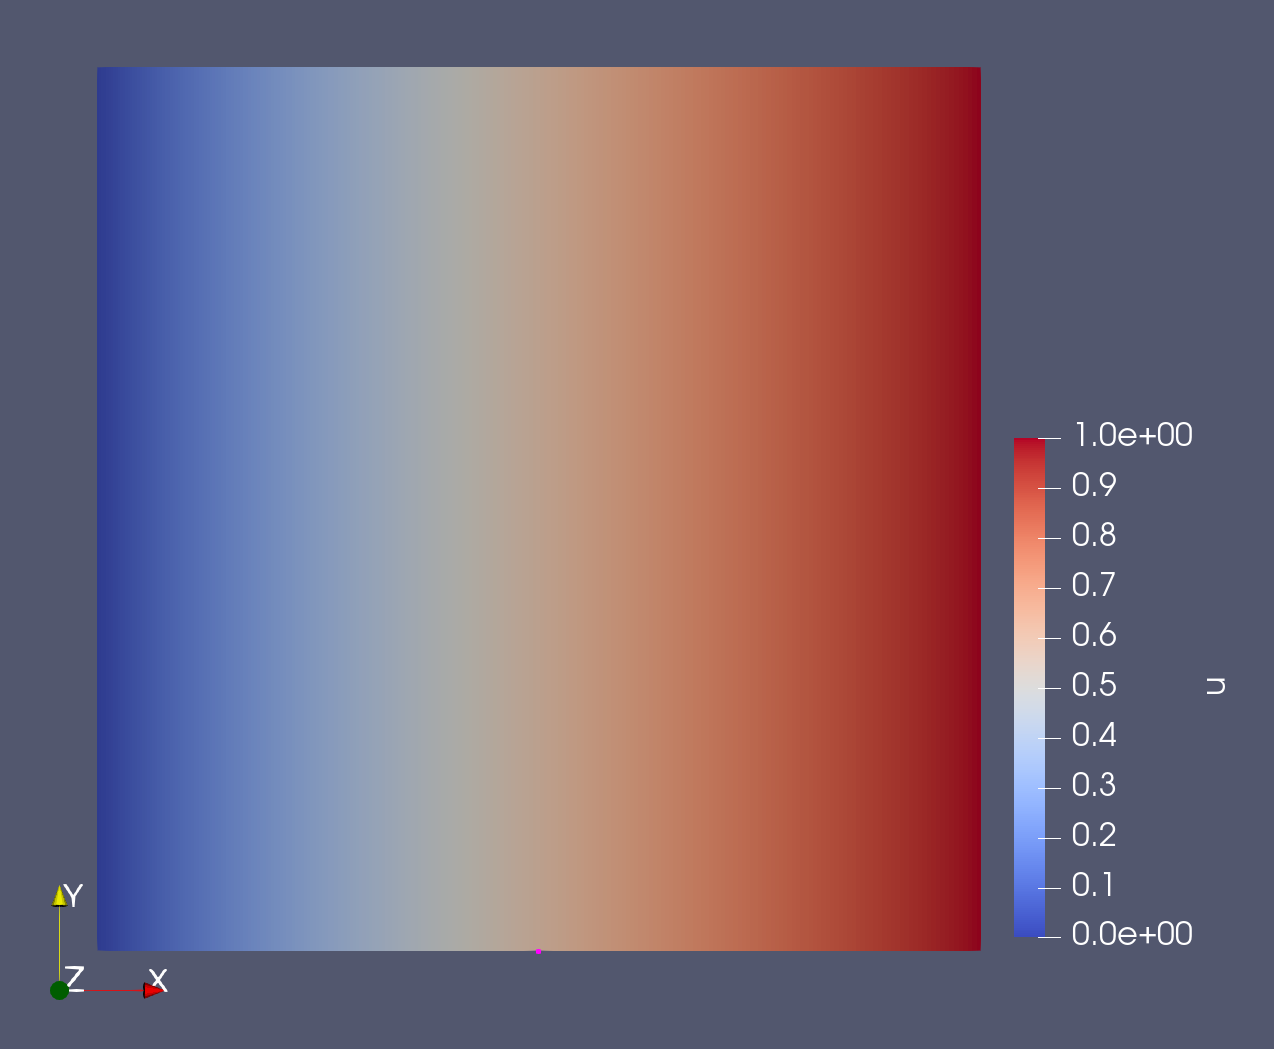
\includegraphics[width=0.6\textwidth]{Figures/result.png}
	\caption{Illustration of the solution of Nonlinear Poisson problem.}
	\label{fig_Rs}
\end{figure}
\begin{table}
	\caption{Illustration of the domain of Poisson problem.}
	\label{tab1}
\begin{center}
	\begin{tabular}{|c| c| c|} 
		\hline
		$x$ & $\mathbf{u}_{numerical}$ & $\mathbf{u}_{exact}$ \\ [0.7ex] 
		\hline\hline
		0 & 0.0 & 0.0 \\  [0.2ex] 
		\hline
		0.2 & 0.26491 & 0.264911064 \\ [0.2ex] 
		\hline
		0.4 & 0.48324 & 0.483239697 \\ [0.2ex] 
		\hline
		0.6 & 0.67332 & 0.673320053 \\ [0.2ex] 
		\hline
		0.8 & 0.84391 & 0.843908891 \\ [0.2ex] 
		\hline
		1.0 & 1.0 & 1.0 \\ [0.2ex] 
		\hline
	\end{tabular}
\end{center}
\end{table}
 
\bibliographystyle{unsrt}
\bibliography{ref}
\end{document}
